\documentclass[a4paper,12pt,reqno]{amsart}
\usepackage{graphicx}
\usepackage{macros_M53}

% pour voir les solutions il faut enlever le commentaire de la ligne suivante
% \solutionstrue

\begin{document}

% ==================================
\hautdepage{

\ifsolutions{Solutions de l'interrogation}\else{Interrogation}\fi\par\normalfont\normalsize
22 novembre 2016\\{[ durée: 1 heure ]}\par
}
% ==================================
\ifsolutions\else
% {\fontencoding{U}\fontfamily{futs}\selectfont\char 66\relax}
\tikz[baseline=(e.base)]{\NoAutoSpacing\node(e){!};\draw[red,ultra thick,line join=round,yshift=-.15ex](90:1em)--(210:1em)--(330:1em)--cycle;}
\textbf{Aucun document n'est autorisé.}

\vspace{14mm}
\fi

%-----------------------------------
\begin{exo}

  On se place dans l'espace vectoriel $M_2(\mathbb{R})$ des matrices $2\times 2$ muni du produit scalaire standard, c.-à-d. pour lequel la base canonique est une base orthonormée et tel que $\scalprod{A}{B} = \tr(A^{\,t}\!B)$. Soit
  $$
    \ens{H}=\big\{ M \in M_2(\mathbb{R}) \big| \tr(M)=1 \big\}
  $$
  l'ensemble des matrices à trace égale à $1$.
  \begin{enumerate}
    \item On note $\id$ la matrice identité de $M_2(\mathbb{R})$. Montrer que $\ev{H} = \id^{\perp}$, où $\ev{H}$ est la direction de $\ens{H}$.
    \item Soit $A = \begin{psmallmatrix} 1 & 1\\[3pt] 0 & 2 \end{psmallmatrix}$. Déterminer la distance de $A$ à $\ens{H}$.

  \end{enumerate}

\end{exo}

\begin{solution}

  \begin{enumerate}
    \item Comme $\scalprod{A}{B}=\tr(A^{\,t}\!B)$, nous avons $\tr(A) = \scalprod{A}{\id}$. Ainsi, comme la trace est linéaire, $\ens{H}=\tr^{-1}(1)$ est un espace affine de direction
      $$
        \ev{H} = \tr^{-1}(0) = \big\{ M \in M_2(\mathbb{R}) \big| \tr(M)=0 \big\} = \big\{ M \in M_2(\mathbb{R}) \big| \scalprod{A}{\id}=0 \big\} = \id^{\perp}.
      $$
    \item D'après la question précédente on cherche la projection de $A$ sur $\ens{H}$ sous la forme $A+t\id \in \ens{H}$ avec $t \in \mathbb{R}$. Nous avons $\tr(A+t\id)=1$ $\Leftrightarrow$ $3+2t=1$ $\Leftrightarrow$ $t=-1$. Ainsi la projection de $A$ sur $\ens{H}$ est $A-\id$ et la distance de $A$ à $\ens{H}$ est égale à $\d(A,A-\id)=\norm{\id}=\sqrt{1^{2}+0^{2}+0^{2}+1^{2}} = \sqrt{2}$.\\[7pt]
      \begin{center}
        \usetikzlibrary{decorations.pathreplacing}
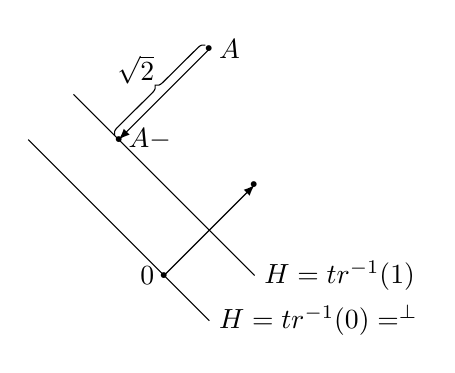
\begin{tikzpicture}[scale=1.15]
  \draw
    (0,0) node[scale=2]{.} node[left]{0}
    (0,0) edge[-latex] (1,1)
    (1,1) node[scale=2]{.} node[right]{$\id$}
      (-1.5,1.5) -- +(2,-2) node[right]{$\ev{H}=tr^{-1}(0)=\id^{\perp}$}
    ++(.5,.5) -- +(2,-2) node[right]{$\ens{H}=tr^{-1}(1)$}
    ++ (.5,-.5) node[scale=2]{.} node[right]{$A-\id$}
      ++(1,1)  coordinate(A) node[scale=2]{.} node[right]{$A$}
    (A) edge[-latex] +(-1,-1)
  ;
   \draw[decorate,decoration={brace,mirror,raise=2pt}] (A) -- node[above left]{$\sqrt{2}$} +(-1,-1);
\end{tikzpicture}

      \end{center}
  \end{enumerate}
\end{solution}

%-----------------------------------
\begin{exo}

  On considère $\mathbb{R}^{2}$ et $\mathbb{R}^{3}$ munis de la structure euclidienne standard. Pour chacune des applications suivantes, déterminer s'il s'agit d'une isométrie, et le cas échéant déterminer sa nature et ses paramètres.

  \begin{enumerate}
    \item $f \in \aff{(\mathbb{R}^{2})}$, $f(x,y)=(\frac{\sqrt{3}}{2}x+\frac{1}{2}y,\frac{1}{2}x-\frac{\sqrt{3}}{2}y+1)$.
    \item $g \in \aff{(\mathbb{R}^{3})}$, $g(x,y,z)=(\frac{1}{\sqrt{2}}x-\frac{1}{\sqrt{2}}z,-y,\frac{1}{\sqrt{2}}x+\frac{1}{\sqrt{2}}z)$.
    \item \textit{[bonus]}\\
    $h \in \aff{(\mathbb{R}^{3})}$, $h=T_{\vv{v}} \circ S_{\ens{H}}$ où $T_{\vv{v}}$ est la translation du vecteur $\vv{v}=(1,1,1)$ et $S_{\ens{H}}$ est la réflexion par rapport au plan $\ens{H}=\{(x,y,z) \in \mathbb{R}^{3} \mid  x+y+z=1\}$.
  \end{enumerate}

\end{exo}

\begin{solution}
  \begin{enumerate}
    \item
      \begin{minipage}[t]{.77\linewidth}
        Nous avons $f(x,y)=A\begin{psmallmatrix} x \\[3pt] y \end{psmallmatrix} + B$ avec
        $ A =
          \begin{psmallmatrix}
            \frac{\sqrt{3}}{2} & -\frac{1}{2} \\[3pt]
            \frac{1}{2} & \frac{\sqrt{3}}{2} \\
          \end{psmallmatrix}
        $ et
        $ B =
          \begin{psmallmatrix}
            0 \\[3pt]
            1 \\
          \end{psmallmatrix}
        $. Comme les vecteurs colonnes de $A$ forment une b.o.n et $\det{A}=-1$, alors $f$ est une réflexion ou une réflexion glissée. Nous avons $f(0,0)=(0,1)$ donc $N=\frac{(0,0)+(0,1)}{2}=(0,\frac12)$ est un point de l'axe de symétrie. De plus $f(N)=(-\frac{1}{4},\frac{\sqrt{3}}{4}+1)=N+\vv{v}$, où $\vv{v}=(-\frac{1}{4},\frac{\sqrt{3}}{4}+\frac12)$.\\
        Ainsi on trouve que $f$ est une réflexion glissée de vecteur $\vv{v}=(-\frac{1}{4},\frac{\sqrt{3}}{4}+\frac12)$ et d'axe passant par $N=(0,\frac12)$ et de direction $\affspan{\vv{v}}$.
      \end{minipage}\hfill
      \begin{minipage}[t]{.21\linewidth}
        ~\\[-14mm] \hspace*{\fill}\scalebox{0.77}{% \def\vv#1{#1}
\usetikzlibrary{calc}
\begin{tikzpicture}[scale=3]
   \path
    (-0.25,0.066987298108) coordinate(v)
    (0,.5) coordinate (N)
    (0,1) coordinate (F0)
    ($(F0)-(v)$) coordinate (S0)
   ;
   \draw[gray] (-.7,0) edge[-latex] (.4,0) (0,-.3) edge[-latex] (0,1.4);
   \draw ($(N)+1.3*(v)$) -- ($(N)-1.5*(v)$);
   \draw[dashed] (0,0) -- (S0) edge[solid,-latex,thick] node[above]{$\vv{v}$} (F0);
   \draw (N) edge[solid,-latex,thick] +(v) +(v) node[scale=2]{.} node[above,xshift=-7mm]{$f(N)=N+\vv{v}$};
   \draw
    (0,0) node[scale=2]{.} node[below left]{$(0,0)$}
    (F0) node[scale=2]{.} node[above left]{$f(0,0)$}
    (N) node[scale=2]{.} node[below left]{$N$}
    (S0) node[scale=2]{.}
   ;
\end{tikzpicture}
}
      \end{minipage}
    \item L'application $g$ est linéaire de la forme $g(x,y,z) = A\begin{psmallmatrix} x \\[3pt] y \\[3pt] z \end{psmallmatrix}$ avec
      $
        A =
        \begin{psmallmatrix}
          \frac1{\sqrt{2}} & 0 & -\frac1{\sqrt{2}} \\[3pt]
          0 & -1 & 0 \\[3pt]
          \frac1{\sqrt{2}} & 0 & \frac1{\sqrt{2}}
        \end{psmallmatrix}
      \in O_{3}^{-}
      $
      car les vecteurs colonnes de $A$ forment une b.o.n. et $\det(A)=-1$. De plus comme $\tr{A}=-1+2\frac1{\sqrt{2}}$ nous déduisons que $g$ est une anti-rotation d'angle $\theta$ tel que $\cos(\theta) = \frac1{\sqrt{2}}$ $\Leftrightarrow$ $\theta=\pm \frac{\pi}{4}$. L'axe de cette rotation est formé par les $(-1)$-vecteurs propres et comme $A\begin{psmallmatrix} 0 \\[3pt] 1 \\[3pt] 0 \end{psmallmatrix} = \begin{psmallmatrix} 0 \\[3pt] \llap{-}1 \\[3pt] 0 \end{psmallmatrix}$, nous obtenons que l'axe est engendré par $\vv{u}=(0,1,0)$ \textit{(et donc le plan de réflexion est le plan d'équation $y=0$)}. Il nous reste à déterminer le signe de l'angle de rotation en orientant l'axe selon $\vv{u}$. Soit $\vv{v}=(1,0,0)$ et $\vv{w}=g(\vv{v})=(\frac1{\sqrt{2}},0,\frac1{\sqrt{2}})$. Comme $\det(u,v,w)=-\frac1{\sqrt{2}} < 0$ nous pouvons conclure que $g$ est une anti-rotation d'axe vectoriel orienté par $(0,1,0)$ et d'angle de rotation $-\frac{\pi}{4}$ autour de cet axe orienté.
    \item Nous avons $\ev{H}=\{(x,y,z) \in \mathbb{R}^{3} \mid  x+y+z=0\} = \vv{v}^{{\perp}}$. Donc d'après le cours $h$ est une réflexion par rapport à un hyperplan (parallèle à $\ens{H}$) de la forme $M+\ev{H}$ où $M$ est un point fixe de $h$. Soit $P=(1,0,0) \in \ens{H}$, ainsi comme $h(P) = T_{\vv{v}} \circ S_{\ens{H}}(1,0,0) = T_{\vv{v}}(1,0,0)=(2,1,1)$ on trouve que $M=\frac{P+h(P)}{2}=(\frac{3}{2},\frac{1}{2},\frac{1}{2})$ convient.\\
    En conclusion $h$ est la réflexion par rapport au plan $\{(x,y,z) \in \mathbb{R}^{3} \mid  x+y+z=\frac{5}{2}\}$ (car $\frac{3}{2}+\frac{1}{2}+\frac{1}{2}=\frac{5}{2}$).\\
    \begin{remarque}
      Une autre rédaction est possible en utilisant que si $\ev{H}\perp\vv{v}$ alors $S_{\ens{H}+\vv{v}/2}\circ S_{\ens{H}} = T_{\vv{v}}$ $\Leftrightarrow$ $T_{\vv{v}}\circ S_{\ens{H}} = S_{\ens{H}+\vv{v}/2}$.
    \end{remarque}
  \end{enumerate}
\end{solution}

\end{document}
